% -*- mode: fundamental -*-

% ****************************************************************

\chapter{The core functions for RISC-V execution}

\markboth{Ch \arabic{chapter}: Core functions (DRAFT)}{\copyrightnotice}

\setcounter{page}{1}
% \renewcommand{\thepage}{\arabic{page}}
\renewcommand{\thepage}{\arabic{chapter}-\arabic{page}}

\label{ch_core_functions}

% ****************************************************************

\section{Introduction}

In this chapter we discuss the core functions of
Figure~\ref{Fig_Simple_Instr_Exec_w_structs}, which we repeat here for
convenience (all the \verb|struct| declarations can be found in the
file: \verb|src_Common/Inter_Stage.bsv|).
\begin{figure}[htbp]
  \centerline{\includegraphics[width=6in,angle=0]{ch030_RISCV_Design_Space/Figures/Fig_Instr_Exec_w_structs}}
  \caption{\label{Fig_Fetch_function_Simple_Instr_Exec}Simple interpretation of RISC-V instructions (same as Fig.~\ref{Fig_Instr_Exec}, with arrows annotated with {\tt struct} types)}
\end{figure}

% ****************************************************************

\section{RISC-V: The Fetch function}

\label{Sec_Fetch_function}

\index{fn\_F@{\tt fn\_F} (Fetch function)}
\index{Fetch function ({\tt fn\_D})}

The Fetch function \emph{per se} is fairly simple, even trivial.  Its
input is the current value of the program counter (PC), which is used
as the address in a memory-request to IMem.  It has two outputs,

\begin{tightlist}

 \item A \emph{memory request} to memory, to read an instruction.  We
   have already seen the definitition of the \verb|Mem_Req| struct in
   the previous chapter.

 \item Some additional information ``\verb|F_to_D|'' passed on to the
 Decode step.

\end{tightlist}

The ``\verb|F_to_D|'' struct has only one interesting field, the PC:

\begin{Verbatim}[frame=single, numbers=left]
typedef struct {
   Bit #(XLEN) pc;
} F_to_D
deriving (Bits, FShow);
\end{Verbatim}

\index{BSV!struct@{\tt struct}!Single-field structs}

\vspace*{2ex}

NOTE:
\fbox{\small
\begin{minipage}{5in}

{\bf BSV: single-field structs}

It might seem like overkill to define a struct for just one field like
the PC (why not just pass the PC?), but it has the following advantages:

\begin{itemize}

  \item It becomes easy to add more fields later, should we need to do
    so.  In particular, for Fife we will need to add some
    branch-prediction information.  We may also wish to add temporary
    fields that aid in debugging.

  \item Stronger type-checking: each new struct type is distinct from
    all other types in a BSV program.  Thus, the type-checker will
    catch any error where we may inadvertantly pass some unrelated and
    irrelevant XLEN-wide value in place of an {\tt F\_to\_D} struct.

  \item There is \emph{no} runtime cost: an {\tt F\_to\_D} value
    occupies the same XLEN bits as the {\tt pc} field by itself.

\end{itemize}

\end{minipage}}

\vspace*{2ex}

\index{BSV!struct!Nested}

To pass both results of \verb|fn_F|, we simply use a \emph{nested}
struct, {\ie} a struct containing the two component structs:

\begin{Verbatim}[frame=single, numbers=left]
typedef struct {
   F_to_D   to_D;        // info to Decode step
   Mem_Req  mem_req;     // requst info to memory
} Result_F
deriving (Bits, FShow);
\end{Verbatim}

Finally, as mentioned earlier, the function \verb|fn_F| is almost
trivial:

\begin{Verbatim}[frame=single, numbers=left]
function Result_F fn_F (Bit #(XLEN)  pc)
   let y = Result_F {to_D: F_to_D {pc: pc},
                     mem_req: Mem_Req {req_type: MEM_LOAD,
                                       size:     MEM_4B,
                                       addr:     pc,
                                       data :    ?}};
   return y;
endfunction
\end{Verbatim}

% ================================================================

\hdivider

% ----------------
\Exercise

Write a testbench for \verb|fn_F()|, apply it to a number of 32-bit
values (PC values) and print the results using \verb|$display| and
\verb|fshow|, and visually check that the \verb|F_to_D| and
\verb|Mem_Req| outputs look correct.

\Endexercise

% ****************************************************************

\section{RISC-V: The Decode function}

\label{Sec_Combo_Decode}

\index{fn\_D@{\tt fn\_D} (Decode function)}
\index{Decode function ({\tt fn\_D})}

The core function for the Decode step is called \verb|fn_D|.  It's
arguments are an \verb|F_to_D| struct from the Fetch step and a
\verb|Mem_Rsp| memory response struct from memory.  It's output struct
type , \verb|D_to_RR|, was described in
Section~\ref{Sec_struct_D_to_RR}.  The code for \verb|fn_D| is mostly
a big if-then-else that analyses the incoming instruction and produces
some summary information:

\begin{Verbatim}[frame=single, numbers=left]
function D_to_RR
         fn_D (F_to_D  x_F_to_D, Mem_Rsp  rsp_IMem);

   Bit #(32) instr = truncate (rsp_IMem.data);
   Bit #(5)  rd    = instr_rd (instr);

   let fallthru_pc = x_F_to_D.pc + 4;

   // Baseline info to next stage
   let y = D_to_RR {pc:           x_F_to_D.pc,

                    exception:    False,
                    cause:        ?,

                    // not-exception
                    fallthru_pc: fallthru_pc,
                    instr:       instr,
                    opclass:     ?,
                    has_rs1:     False,
                    has_rs2:     False,
                    has_rd:      False,
                    writes_mem:  False,
                    imm:         0};

   if (rsp_IMem.rsp_type == MEM_RSP_MISALIGNED) begin
      y.exception = True;
      y.cause     = cause_INSTRUCTION_ADDRESS_MISALIGNED;
   end
   else if (rsp_IMem.rsp_type == MEM_RSP_ERR) begin
      y.exception = True;
      y.cause     = cause_INSTRUCTION_ACCESS_FAULT;
   end
   else if (is_legal_LUI (instr) || is_legal_AUIPC (instr)) begin
      y.opclass = OPCLASS_IALU;
      y.has_rd  = non_zero_rd;
      y.imm     = zeroExtend (instr_imm_U (instr));
   end
   else if (is_legal_BRANCH (instr)) begin
      y.opclass = OPCLASS_CONTROL;
      y.has_rs1 = True;
      y.has_rs2 = True;
      y.imm     = zeroExtend (instr_imm_B (instr));
   end
   else if (is_legal_JAL (instr)) begin
      y.opclass = OPCLASS_CONTROL;
      y.has_rd  = non_zero_rd;
      y.imm     = zeroExtend (instr_imm_J (instr));
   end
   else if (is_legal_JALR (instr)) begin
      y.opclass = OPCLASS_CONTROL;
      y.has_rs1 = True;
      y.has_rd  = non_zero_rd;
      y.imm     = zeroExtend (instr_imm_I (instr));
   end
   else if (is_legal_LOAD (instr)) begin
      y.opclass = OPCLASS_MEM;
      y.has_rs1 = True;
      y.has_rd  = non_zero_rd;
      y.imm     = zeroExtend (instr_imm_I (instr));
   end
   else if (is_legal_STORE (instr)) begin
      y.opclass    = OPCLASS_MEM;
      y.has_rs1    = True;
      y.has_rs2    = True;
      y.writes_mem = True;
      y.imm        = zeroExtend (instr_imm_S (instr));
   end
   else if (is_legal_OP_IMM (instr)) begin
      y.opclass = OPCLASS_IALU;
      y.has_rs1 = True;
      y.has_rd  = non_zero_rd;
      y.imm     = zeroExtend (instr_imm_I (instr));
   end
   else if (is_legal_OP (instr)) begin
      y.opclass = OPCLASS_IALU;
      y.has_rs1 = True;
      y.has_rs2 = True;
      y.has_rd  = non_zero_rd;
   end
   else if (is_legal_ECALL (instr) || is_legal_EBREAK (instr)) begin
      y.opclass = OPCLASS_SYSTEM;
   end
   else if (is_legal_FENCE (instr) || is_legal_FENCE_I (instr)) begin
      y.opclass = OPCLASS_FENCE;
      y.has_rs1 = True;
      y.has_rd  = non_zero_rd;
   end
   else begin
      y.exception = True;
      y.cause     = cause_ILLEGAL_INSTRUCTION;
   end

   return y;
endfunction
\end{Verbatim}

In line 4, we extract the instruction from the \verb|Mem_Rsp| memory
response from the Fetch operation, and in line 5 we extract the
\verb|rd| (``destination register'') field from the instruction.

\index{truncate@{\tt truncate}, operation to shrink bit-width}

In line 4, the \verb|truncate| operation is used to shrink the
bit-vector width of \verb|rsp_IMem.data| to the bit-vector width of
\verb|instr| (32-bits).  But why is this shrinkage needed?  After all,
in the declaration of the \verb|Mem_Rsp| type, the \verb|data| field
is declared to have type \verb|Bit#(XLEN)| which is synonymous with
\verb|Bit#(32)|.  The reason is that we've written the code to be
ready for re-use in the future with RV64, when \verb|XLEN| will be
defined as 64.  The \verb|truncate| operation is polymorphic,
accepting arguments of any bitwidth wider than the required output.
Here, when the argument is 32-bits wide, it does nothing (is a no-op);
but for RV64, when the argument is 64-bits wide, it performs the
shrinkage to 32 bits.  Note, \verb|truncate| keeps least-significant
bits and drops most-significant bits.

In line 7 we compute the fall-through PC, PC+4 (with the caveat that
if we want to support the ``C'' RISC-V ISA extension (``Compressed''
instructions), it may be PC+2, which information can be gleaned from
the instruction encoding).

In lines 10-23 we create a baseline \verb|D_to_RR| value which we will
selectively modify in the if-then-elses below.

In lines 25-32 we first handle the sitation where the Fetch operation
to memory itself returned an error.  We mark the \verb|exception|
field True and fill in the appropriate \verb|cause|.

The rest of the code is a series of if-then-else clauses. Each clause
identifies one class of instruction and updates the \verb|opclass|
field correspondingly.  The repertoire of instructions that we
consider are the forty instructions listed in the ``RV32I Base
Instruction Set'' table of ``Table 24.2: Instruction listing for
RISC-V'' of the Unprivileged Spec~\cite{RISCV_Unpriv_2019_12_13}.

Each if-then-else clause also fills in the \verb|has_rs1|,
\verb|has_rs2| and \verb|has_rd| fields, as appropriate, for each
class of instruction.  We also decode each kind of ``immediate'' field
and fill in the \verb|imm| field.

The final ``else'' clause (lines 88-91) is evaluated if the
instruction does not match one of the forty RV32I instructions.  In
this case we set the \verb|exception| and \verb|cause| fields to
indicate an illegal instruction.

Note the use of functions \verb|instr_imm_I()|, \verb|instr_imm_S()|,
\verb|instr_imm_B()|, \verb|instr_imm_U()| and \verb|instr_imm_J()|,
which extract the ``immediate'' field from a 32-bit instruction.  For
the different classes of instruction (I, S, B, U, J), the immediates
are coded differently, and have different widths (see the schemata at
the top of the RV32I page in ``Table 24.2: Instruction listing for
RISC-V'' of the Unprivileged Spec~\cite{RISCV_Unpriv_2019_12_13}).
These functions decode the bits and zero-extend them to XLEN bits (the
width of \verb|d_to_rr.imm|).  Later, in the ``execute'' code for each
instruction, we will pick out the relevant bits out of the XLEN bits,
and zero-extend or sign-extend them as needed for the particular
instruction.

An exercise below suggests that you write the code for these
\verb|instr_imm_X| functions; it's good practice for the BSV beginner!

Observe that the entire \verb|fn_D()| function is just a (large)
combinational circuit---it is an acyclic composition of smaller
combinational circuits, many of which we've seen earlier.  The whole
\verb|fn_D()| function can be visualized as a box with incoming wires
corresponding to \verb|F_to_D| and \verb|Mem_Rsp|, outgoing wires
corresponding to \verb|D_to_RR|, and filled with logic gates that
compute each output wire as a function of the input wires.

% ================================================================

\hdivider

% ----------------
\Exercise

Write the functions \verb|instr_imm_I()|, \verb|instr_imm_S()|,
\verb|instr_imm_B()|, \verb|instr_imm_U()| and \verb|instr_imm_J()|.

% ----------------
\Exercise

Write a testbench for \verb|fn_D()|, apply it to a number of PC and
instruction values.  For each input PC value, construct an
\verb|F_to_D| struct around it.  For each input instruction, construct
a \verb|Mem_Rsp| struct around it, some with memory errors, some
without.  Apply \verb|fn_D| to such pairs.  Print the results results
using \verb|$display| and \verb|fshow|, and visually check that the
\verb|D_to_RR| outputs look correct.

\Endexercise

% ****************************************************************

\section{RISC-V: The Execute Control function}

\label{Sec_fn_Control}

\index{fn\_Control@{\tt fn\_Control} (Execute Control function)}
\index{Execute Control function ({\tt fn\_Control})}

Having discussed the Fetch and Decode functions, we will next discuss
the ``execute'' functions (Control, IALU and DMem), which can also be
characterized as pure value-to-value functions.  We will return to the
Register Read (RR) and Retire steps in later chapters.

The input and output of \verb|fn_Control|, the Control function in
Figure~\ref{Fig_Simple_Instr_Exec_w_structs}, are values of the
following types, respectively.  Each of the input fields is needed to
compute one or more of the output fields.

{\small
\begin{Verbatim}[frame=single, numbers=left]
typedef struct {Bit #(XLEN)  pc;
		Bit #(XLEN)  fallthru_pc;
		Bit #(32)    instr;
		Bit #(XLEN)  rs1_val;
		Bit #(XLEN)  rs2_val;
		Bit #(32)    imm;
} RR_to_Control
deriving (Bits, Eq, FShow);

typedef struct {Bool         exception;
		Bit #(XLEN)  cause;        // Misaligned BRANCH/JAL/JALR target

		Bit #(XLEN)  next_pc;
		Bool         data_valid;    // True for JAL/JALR; False for BRANCH
		Bit #(XLEN)  data;          // Return-PC for JAL/JALR
} Control_to_Retire
deriving (Bits, FShow);
\end{Verbatim}
}

Here is the Control function \verb|fn_Control|:

{\small
\begin{Verbatim}[frame=single, numbers=left]
function Control_to_Retire fn_Control (RR_to_Control  x);
   let instr   = x.instr;
   let rs1_val = x.rs1_val;
   let rs2_val = x.rs2_val;

   Bit #(XLEN)  next_pc   = ?;
   Bool         exception = False;    // Misaligned target_pc

   if (is_BRANCH (instr)) begin
      Bool branch_taken = case (instr_funct3 (instr))
                             funct3_BEQ:  (rs1_val == rs2_val);
                             funct3_BNE:  (rs1_val != rs2_val);
                             funct3_BLT:  signedLT (rs1_val, rs2_val);
                             funct3_BGE:  signedGE (rs1_val, rs2_val);
                             funct3_BLTU: (rs1_val < rs2_val);
                             funct3_BGEU: (rs1_val >= rs2_val);
                          endcase;
      Bit #(13) imm13 = x.imm [12:0];
      let target_pc = x.pc + signExtend (imm13);
      next_pc = (branch_taken ? target_pc : x.fallthru_pc);
      exception = (branch_taken && (target_pc [1:0] != 0));
   end
   else if (is_JAL (instr)) begin
      Bit #(21) imm21 = x.imm [20:0];
      next_pc = x.pc + signExtend (imm21);
      exception = (next_pc [1:0] != 0);
   end
   else if (is_JALR (instr)) begin
      Bit #(12) imm12 = x.imm [11:0];
      // zero out LSB in target PC
      next_pc = ((rs1_val + signExtend (imm12)) & ~1);
      exception = (next_pc [1:0] != 0);
   end

   Bool data_valid = ((instr_rd  (instr) != 0)
                      && (is_JAL (instr) || is_JALR (instr)));
   let y = Control_to_Retire {inum:       x.inum,
                              pc:         x.pc,
                              instr:      x.instr,
                              exception:  exception,
                              cause:      cause_INSTRUCTION_ADDRESS_MISALIGNED,
                              next_pc:    next_pc,
                              data_valid: data_valid,
                              data:       x.fallthru_pc};
   return y;
endfunction
\end{Verbatim}
}

Lines 9-22 handle BRANCH (conditional branch) instructions.  First the
\verb|case| expression computes the boolean value \verb|branch_taken|,
the decision whether to take the branch or not.  This is based on the
3-bit \verb|funct3| field of the instruction that identifies the
specific condition to be tested.  Note that for BLT and BGE, we use
the \verb|signedLT| and \verb|signedGE| functions that interpret
\verb|rs1_val| and \verb|rs2_val| as signed integers.

Line 19 computes the target PC should the the branch be taken.  Line
20 computes the next PC, which is either the target PC or the
fall-through PC depending on whether the branch is taken or not.
Finally, Line 21 checkes that if the branch is taken, that the target
PC is a suitably aligned address.

Lines 23-27 handle JAL (Jump and Link) instructions, and lines 28-33
handle the JALR (Jump and Link Register) instructions.  They are both
straightforward, unconditional calculations of a next PC, along with
an alignment-check that the next PC is suitably aligned.

Notice that the nested if-then-else has no final ``else'' clause.
This is safe because of the checks already done in the Decode function
\verb|Fn_D|, which guarantee that this function will only be invoked
with inputs that are handled by one of the three clauses.

Finally, lines 35 through 45 construct the final result and return it.

\vspace*{2ex}

NOTE:
\fbox{\small
\begin{minipage}{5in}

{\bf RISC-V: misaligned branch/jump targets}

\vspace{1ex}

In {\tt fn\_Control}, the BRANCH, JAL and JALR clauses set the
{\tt exception} field to true if the next PC is not aligned.  This is
required by the RISC-V Spec (see ``Section 2.5 Control Transfer
Instructions'' in \cite{RISCV_Unpriv_2019_12_13}).  If there is a
misalignment error, we encounter it here on the control-transfer
instruction.

\vspace{1ex}

If we do not check alignment here, we will encounter a misalignment
error on the next Fetch, at the next-PC address.  The choice of
catching this earlier, at the control-transfer instruction itself, is
a design choice by the RISC-V ISA architects.

\end{minipage}}

\vspace*{2ex}

\hdivider

% ----------------
\Exercise

Prove (informally) that the three-way if-then-else in
\verb|Fn_Control| will catch all cases, {\ie} that we never need a
final ``else'' clause.  This requires reviewing the Decode function
\verb|fn_D|, and tracking the flow of information through the
Register-Read function \verb|fn_RR| into \verb|fn_Control|.

% ----------------
\Exercise

In \verb|Fn_Control|, can we change the final ``if'' condition line:

{\small
\begin{Verbatim}[frame=single]
   else if (is_JALR (instr)) begin
\end{Verbatim}
}

into a simple ``else'' clause ({\ie} omit the the \verb|is_JALR| check)?

{\small
\begin{Verbatim}[frame=single]
   else begin
\end{Verbatim}
}

What might be the hardware implication of such a change?

% ----------------
\Exercise

In line 35 in {\tt fn\_Control}, we are testing {\tt (instr\_rd
(instr) != 0)}.  But we tested this in computing the boolean {\tt
has\_rd} in {\tt fn\_D}, the Decode function.  Discuss the hardware
tradeoffs in just passing that boolean value along in the structs to
this point, instead of recomputing it here.

\Endexercise

% ****************************************************************

\section{RISC-V: The Execute Integer Ops function}

\label{Sec_fn_EXI}

\index{fn\_EX\_IALU@{\tt fn\_IALU} (Execute Integer Ops function)}
\index{Execute Integer Ops function ({\tt fn\_EX\_IALU})}

The input and output of \verb|fn_EX_IALU|, the ``Execute Integer Ops''
function in Figure~\ref{Fig_Simple_Instr_Exec_w_structs}, are values
of the following types, respectively.  Each of the input fields is
needed to compute one or more of the output fields.

{\small
\begin{Verbatim}[frame=single, numbers=left]
typedef struct {Bit #(XLEN)  pc;
		Bit #(32)    instr;
		Bit #(XLEN)  rs1_val;
		Bit #(XLEN)  rs2_val;
		Bit #(32)    imm;
} RR_to_EX
deriving (Bits, FShow);

typedef struct {Bool         exception;
		Bit #(XLEN)  cause;

		Bool         data_valid;
		Bit #(XLEN)  data;
} EX_to_Retire
deriving (Bits, FShow);
\end{Verbatim}
}

Here is the Execute Integer Ops function \verb|fn_EX_IALU|:

{\small
\begin{Verbatim}[frame=single, numbers=left]
function EX_to_Retire fn_EX_IALU (RR_to_EX x);
   let instr = x.instr;

   let y = EX_to_Retire {inum:       x.inum,
                         pc:         x.pc,
                         instr:      instr,
                         exception:  False,
                         cause:      ?,
                         data_valid: True,
                         data:       ?};

   if (is_LUI (instr))
      y.data = (zeroExtend (instr_imm_U (instr)) << 12);
   else if (is_AUIPC (instr)) begin
      Bit #(XLEN) offset = signExtend ({ instr_imm_U (instr), 12'b0 });
      y.data = x.pc + offset;
   end
   else begin
      let result <- fn_IALU (logf, instr, x.rs1_val, x.rs2_val, x.imm);
      y.data = result;
   end
   return y;
endfunction
\end{Verbatim}
}

Lines 12-13 handle LUI instructions (Load Upper Immediate).  Lines
14-17 handle AUIPC instructions (Add Upper Immediate to PC).  Lines
18-21 invoke {\tt fn\_IALU} to perform all the remaining Integer ops,
and this is shown in the code below.

{\small
\begin{Verbatim}[frame=single, numbers=left]
function Bit #(XLEN) fn_IALU (Bit #(32)    instr,
                              Bit #(XLEN)  v1,
                              Bit #(XLEN)  v2,
                              Bit #(32)    imm);
   Bit #(7)    opcode = instr_opcode (instr);
   Bit #(3)    funct3 = instr_funct3 (instr);
   Int #(XLEN) iv1    = unpack (v1);
   Int #(XLEN) iv2    = unpack (v2);
   Int #(XLEN) i_imm  = unpack (signExtend (instr_imm_I (instr)));

   Bit #(XLEN) y_OP     = 0;
   if (opcode == opcode_OP) begin
      Bit #(5) shamt = v2 [4:0];
      case (funct3)
         funct3_ADD:  y_OP = pack ((instr [30] == 1'b0)
	                           ? (iv1 + iv2)
				   : (iv1 - iv2));
         funct3_SLL:  y_OP = v1 << shamt;
         funct3_SLT:  y_OP = ((iv1 < iv2) ? 1 : 0);
         funct3_SLTU: y_OP = ((v1  < v2)  ? 1 : 0);
         funct3_XOR:  y_OP = v1 ^ v2;
         funct3_SRL:  y_OP = v1 >> shamt;
         funct3_SRA:  y_OP = pack (iv1 >> shamt);
         funct3_OR:   y_OP = v1 | v2;
         funct3_AND:  y_OP = v1 & v2;
      endcase
   end

   Bit #(XLEN) y_OP_IMM = 0;
   if (opcode == opcode_OP_IMM) begin
      Bit #(5) shamt = imm [4:0];
      case (funct3)
         funct3_ADDI:  y_OP_IMM = pack (iv1 + i_imm);
         funct3_SLTI:  y_OP_IMM = ((iv1 < i_imm) ? 1 : 0);
         funct3_SLTIU: y_OP_IMM = ((v1  < imm)   ? 1 : 0);
         funct3_XORI:  y_OP_IMM = v1 ^ imm;
         funct3_ORI:   y_OP_IMM = v1 | imm;
         funct3_ANDI:  y_OP_IMM = v1 & imm;
         funct3_SLLI:  y_OP_IMM = v1 << shamt;
         funct3_SRLI:  y_OP_IMM = v1 >> shamt;
         funct3_SRAI:  y_OP_IMM = pack (iv1 >> shamt);
      endcase
   end

   return (y_OP | y_OP_IMM);
endfunction
\end{Verbatim}
}

In lines 7-8, we define signed-integer versions {\tt iv1}, {\tt iv2}
of the unsigned integer values {\tt v1} and {\tt v2}, respectively.
There is no hardware cost to this definition, it's simply a
declaration to ``view'' the same bits differently (as 2's-complement
coded integers).  The difference arises later, when we apply certain
operators to these values.  For example, lines 19-20 compute the SLT
(Set Less Than (signed)) and SLTU (Set Less Than Unsigned) operations.
The SLT op uses the signed values {\tt iv1} and {\tt iv2}, whereas
SLTU uses the unsigned values {\tt v1} and {\v2}.  Between the
\emph{bsc} compiler and the Verilog back-end, different code will be
generated for the ``{\tt <}'' operator to perform the correct kind of
comparison.

Line 13 extracts a 5-bit ``shift amount'' from the {\tt rs2} value for
the shift operators SLL, SRL and SRA.  Line 31 extract a 5-bit ``shift
amount'' from the {\tt imm} value for the shift operators SLLI, SRLI
and SRAI.  SRL (Shift Right Logical) and SRA (Shift Right Arithmetic)
differ in whether they treat the argument as a signed or unsigned
value, the difference being whether the new bits shifted in at the
most-significant bit side are zero (SRL) or replicate the
most-significant bit (SRA).  SRLI and SRAI exhibit a similar
difference.

In lines 23 (SRA) and 41 (SRAI) we finally apply the ``{\tt pack}''
operator to produce the result. This is because the expression
``\verb|(iv1 >> shamt)|'' has type {\tt Int\#(XLEN)} whereas the
result needs to be of type {\tt Bit\#(XLEN)}.  The ``{\tt pack}''
operator performs this type-change for us.

Lines 11-27 define the {\tt y\_OP} result when the opcode is {\tt
opcode\_OP} {\ie} {\tt 7'b\_011\_0011}, {\ie} the ``3-address''
operators where the inputs come from {\tt rs1} and {\tt rs2}.
It defaults to 0 when it is not an {\tt op\_OP}.

Lines 29-43 define the {\tt y\_OP\_IMM} result when the opcode is {\tt
opcode\_OP\_IMM} {\ie} {\tt 7'b\_001\_0011}, {\ie} the ``2-address''
operators where one input come from {\tt rs1} and the other input
comes from an immediate value in the instruction.
It defaults to 0 when it is not an {\tt op\_OP\_IMM}.

Finally, line 45 combines these results using the ``OR'' function.  We
rely on the fact that exactly one of \verb|y_OP| and \verb|y_OP_IMM|
can be relevant; the other one must be zero (and therefore has no
effect through the OR'ing).

\hdivider

% ----------------
\Exercise

Lines 11-45 could instead have been written this way:

{\small
\begin{Verbatim}[frame=single, numbers=left]
   Bit #(XLEN) y = 0;
   if (opcode == opcode_OP) begin
      ...
      ... y = ...
   end
   else if (opcode == opcode_OP_IMM) begin
      ...
      ... y = ...
   end
   return y;
\end{Verbatim}
}

Discuss the hardware tradeoffs between writing it in these two ways.
{\emph Hints:} Consider:

\begin{tightlist}

  \item Sequentiality of if-then-else.
  \item Ability (or not) to prove exhaustiveness of conditions in nested if-then-else.
  \item Ability (or not) to prove mutual-exclusivity of conditions in nested if-then-else.
  \item Discussion in Section~\ref{Sec_MUXes} on parallel and
    sequential multiplexers (mux).  Note: in our code, we have
    explicitly coded a parallel mux.

\end{tightlist}

% ----------------
\Exercise

Note that the ISA has ADD and ADDI instructions, but no corresponding
SUB and SUBI (subtract) instructions.  Why not?

% ----------------
\Exercise

Justify the presence or absence of the ``{\tt pack}'' operator in each
case of {\tt fn\_IALU}.

% ----------------
\Exercise

Suppose we want to extend {\tt fn\_IALU} so it also works when XLEN=64
({\ie} for RV64I).  What needs to change to accommodate this?

\emph{Hint:} it only matters in the shift-amount of the shift
instructions, where the shift-amount can be 6-bits wide instead of
5-bits (allowing a maximum of 63-bit shifts instead of 31 bits).

\Endexercise

% ****************************************************************

\section{RISC-V: The Execute DMem function}

\label{Sec_fn_DMem}

\index{fn\_DMem@{\tt fn\_DMem} (Execute DMem function)}
\index{Execute DMem function ({\tt fn\_DMem})}

The types of the input and output of the ``Execute Memory Ops''
function in Figure~\ref{Fig_Simple_Instr_Exec_w_structs} are the same
as for ``Execute Integer Ops'', {\ie} {\tt RR\_to\_EX} and {\tt
EX\_to\_Retire}, which were described in Section~\ref{Sec_fn_EXI}.

Figure~\ref{Fig_fn_DMem} shows that the ``Execute Memory Ops''
function can be split into two phases,
\begin{figure}[htbp]
  \centerline{\includegraphics[width=6in,angle=0]{ch060/Figures/Fig_fn_DMem}}
  \caption{\label{Fig_fn_DMem}The Execute Memory Ops function is split into two phases.}
\end{figure}
just like we did for Fetch.  The first phase generates a memory
request, and the second phase processes the memory response.  As with
Fetch, there is no guarantee how ``soon'' the response will come.

Here is the function for the first phase, computing a memory request:
{\small
\begin{Verbatim}[frame=single, numbers=left]
function Mem_Req fn_DMem_Req (RR_to_EX  x);
   Bool is_LD = is_LOAD  (x.instr);
   Bool is_ST = is_STORE (x.instr);

   // Mem effective-address calculation
   Int #(XLEN) ibase   = unpack (x.rs1_val);                  // Signed
   Int #(XLEN) ioffset = unpack (signExtend (x.imm [11:0]));  // Signed
   Bit #(XLEN) eaddr   = pack (ibase + ioffset);

   Mem_Req_Size mrq_size = unpack (x.instr [13:12]);  // B, H, W or D
   Mem_Req_Type mrq_type = (is_LD ? funct5_LOAD : funct5_STORE);

   let y = Mem_Req {inum:     x.inum,
                    pc:       x.pc,
                    instr:    x.instr,
                    req_type: mrq_type,
                    size:     mrq_size,
                    addr:     zeroExtend (eaddr),
                    data :    zeroExtend (x.rs2_val)};
   return y;
endfunction
\end{Verbatim}
}

Lines 6-8 compute the so-called ``Effective Address'' of a LOAD/STORE,
by performing a \emph{signed} addition of the {\tt rs1} and immediate
values.

Line 10 defines the memory-request size (1, 2, 4 or 8 bytes), which in
RISC-V terminology are referred to as Bytes (B), Halfwords (H), Words
(W) and Doublewords (D), respectively).  The {\tt Mem\_Req\_Size} type
is defined in the file {\tt Mem\_Req\_Rsp.bsv} as follows:

{\small
\begin{Verbatim}[frame=single, numbers=left]
typedef enum {MEM_1B, MEM_2B, MEM_4B} Mem_Req_Size
deriving (Eq, FShow, Bits);
\end{Verbatim}
}

Line 10 relies on the fact that these will be coded as 2'b00, 2'b01
and 2'b10, which is exactly the coding found in {\tt instr[13:12]}, so
we can simply ``{\tt unpack}'' the bits to the type {\tt
Mem\_Req\_Size} without any further manipulation.

% ----------------
\hdivider

\Exercise

In Line 10, what if {\tt instr[13:12]} had the value 2'b11?  This is a
legal instruction in the RV64I ISA, for LOADs and STOREs of 8-byte
values, but illegal in RV32I.  Should we check that here?

\emph{Hint:} study the {\tt is\_legal\_LOAD()} {\tt
is\_legal\_STORE()} functions used in the Decode function {\tt
fn\_D()} to see if we will ever encounter an illegal value here.

\Exercise

Write a different version of Line 10 that does not rely on the
one-to-one coding equivalence of {\tt instr[13:12]} and the bit coding
of {\tt Mem\_Req\_Size}.

\emph{Hint:} The solution will be a nested if-then-else, or a {\tt
case} expression.

\Endexercise
% ----------------

Here is the function for the second phase, accepting a memory response
as argument and computing the struct to be sent to the Retire step.

{\small
\begin{Verbatim}[frame=single, numbers=left]
function EX_to_Retire fn_DMem_Rsp (Mem_Rsp x);
   Bool exception = ((x.rsp_type == MEM_RSP_ERR)
                     || (x.rsp_type == MEM_RSP_MISALIGNED));
   Bit #(XLEN)  cause = ((x.rsp_type == MEM_RSP_MISALIGNED)
       		      	 ? (is_LOAD (x.instr)
			    ? cause_LOAD_ADDRESS_MISALIGNED
			    : cause_STORE_AMO_ADDRESS_MISALIGNED)
			 : (is_LOAD (x.instr)
                            ? cause_LOAD_ACCESS_FAULT
                            : cause_STORE_AMO_ACCESS_FAULT));

   let y = EX_to_Retire {exception:  exception,
                         cause:      cause,

                         data_valid: (! is_STORE (x.instr)),
                         data:       truncate (x.data)};
   return y;
endfunction
\end{Verbatim}
}

Lines 2-10 convert the memory-systems ``exception'' codes ({\tt
MEM\_RSP\_ERR} and {\tt MEM\_RSP\_MISALIGNED}) into RISC-V {\tt cause}
codes ({\tt cause\_...}).)

Lines 12-16 constructs the required {\tt EX\_to\_Retire} result and
line 17 returns it.

Line 15 uses {\tt (!~is\_STORE())} to indicate whether the {\tt data}
field is valid or not, {\ie} if it is not a STORE, it must be a LOAD,
returning data.  Note that the code may set {\tt data\_valid} to true
when there is an exception in a LOAD, but in that case the {\tt
data\_valid} value does not matter.

% ----------------
\hdivider

\Exercise

When implementing the ``A'' RISC-V ISA Extension (Atomic Memory Ops),
the repertoire of memory operations widens from LOAD and STORE to
include LR (Load-Reserved), SC (Store-Conditional) and a variety of
AMOxxx ops such as AMOADD, AMOSWAP, and so on.
Will line 15's {\tt (!~is\_STORE())} remain adequate, in that case?

\Endexercise
% ----------------

% ****************************************************************

\section{RISC-V: The Register-Read function}

\label{Sec_fn_RR}

\index{fn\_RR@{\tt fn\_RR} (Register-read function)}
\index{Register-read function ({\tt fn\_RR})}

% ****************************************************************

\section{RISC-V: The Retire function}

\label{Sec_fn_Retire}

\index{fn\_Retire@{\tt fn\_Retire} (Retire function)}
\index{Retire function ({\tt fn\_Retire})}

% ****************************************************************
